\section{Personas}\label{l:personas}

\begin{table}
\begin{center}
\begin{tabular}{@{}l l}
\textbf{Projektleiter} &\\
\hline
Arthur Blozyk & Sales Information and Communication\\ 
& \emph{MAN Truck \& Bus AG}\\
Sebastian Nell & Director of USE // Connected Products\\
& \emph{Scholz \& Volkmer GmbH}\\
Tobias Rudolphi	& Lead Software Architect\\
& \emph{Zühlke Engineering GmbH}\\
\textbf{Konzept, Design} &\\
\hline
Carsten Fischer	& UX Designer \& Informationsarchitekt\\
& \emph{triplesense GmbH}\\
Eva Kümml & Senior Konzept / User Experience\\
& \emph{SinnerSchrader Deutschland GmbH}\\
Sandra-Charlotte Hildebrandt & Dipl. Designerin\\
& \emph{selbständig}\\
\textbf{Produktion} &\\
\hline
Sebastian Beyer	& Developer\\
& \emph{Scholz \& Volkmer GmbH}\\
Jan Lochner	& Dipl. Multimedia Producer\\
& \emph{selbständig}\\
\textbf{Texter} &\\
\hline
Marc Stenzel & Freier Projektleiter, Fachjournalist\\
& \emph{selbständig}\\
Torsten Schölzel & Freier Texter und Konzeptioner\\
& \emph{selbständig}\\
\textbf{Übersetzer} &\\
\hline
Jorinde Gessner	& Information Manager\\
& \emph{Ogilvy \& Mather Deutschland GmbH}\\
\textbf{Kunde} &\\
\hline
Markus Rüb & Sales Information and Communication\\
& \emph{MAN Truck \& Bus AG}
\end{tabular}
\caption{Interviewte Personen}
\label{table:interviewpartner}
\end{center}
\end{table}

Im vorigen Abschnitt wurden die Probleme geschildert, die im aktuell üblichen Projektverlauf auftreten und daraus gefolgert, was die wichtigsten Aspekte sind, die eine mögliche Lösung behandeln muss. Um den Entwurf einer Lösung im nächsten Abschnitt vorzubereiten werden in diesem Abschnitt \emph{Personas} vorgestellt, die die typischen Benutzergruppen des Systems repräsentieren und ihre Aufgaben und Erwartungen zusammen fassen. Personas sind ein wichtiger Baustein für den Entwurf eines Systems. Personas ermögliche es, Konzepte und Ideen schon während des Entwurfs zu verfizieren in dem deren Auswirkungen mit dem Nutzungsverhalten und den Erwartungen der Personas verglichen werden.

\begin{quote}
\textit{Personas describe a site’s target users, giving a clear picture of how they’re likely to use the system, and what they’ll expect from it, among other
things. […] Without personas, there is no common language for talking about what users want.} \cite[S.15 ff.]{brown2007communicating}
\end{quote}

Personas bilden nicht nur im Entwurf eine wichtige Entscheidungshilfe sondern werden auch während der Umsetzung immer wieder zu Rate gezogen, in dem neue Funktionalitäten auf deren Relevanz und mögliche Probleme für bestimmte Personas hin überprüft werden. \cite[S.38 ff.]{cohn2004user}

\subsection{Überblick}

\begin{figure}[htb]
\begin{center}
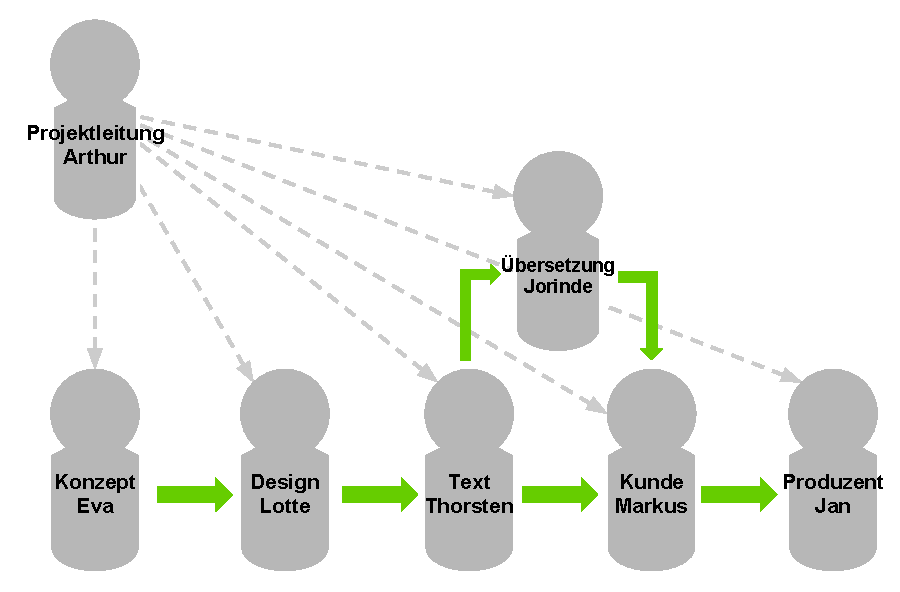
\includegraphics[width=\textwidth]{media/Uebersicht-Personas.pdf}
\caption{Übersicht über die Personas und den idealisierten Workflow}
\label{chart:uebersicht-personas}
\end{center}
\end{figure}

Die nachfolgend vorgestellten Personas basieren auf den im April 2012 geführten Interviews mit den in Tabelle~\ref{table:interviewpartner} auf Seite~\pageref{table:interviewpartner} aufgezählten Personen. Die Auswahl der Personas orientierte sich dabei primäre an dem vorherrschenden Workflow innerhalb der Projekte. Es wurde versucht möglichst eindeutige Rollen zu identifizieren und Überschneidungen zwischen den Personas zu vermeiden. Die folgende Auflistung ist in der Reihenfolge idealisiert -- wie in Abschnitt~\ref{l:problemanalyse} jedoch gezeigt wurde, ergeben sich vielzählige Feedback-Schleifen -- und listet den Einfluss der Beteiligten in Bezug auf die Texte des Produktes.

\begin{enumerate}
\item Die \textbf{Konzeptin \emph{Eva}} entwickelt das Produkt, wobei sie die Rahmenbedingungen wie Aufbau, Umfang, Zielgruppe, Ansprache festlegt. 
\item Die \textbf{Designerin \emph{Lotte}} gestaltet das Produkt, wobei er bestimmt, wie Texte dargestellt werden (Satz, Länge, Schriftart, Farben, Hervorhebungen)
\item Der \textbf{Texter \emph{Thorsten}} erstellt die Texte für das Produkt in der Ausgangssprache
\item Der \textbf{Kunde \emph{Markus}} nimmt die Texte ab
\item Die \textbf{Übersetzerin \emph{Jorinde}} übersetzt die Texte
\item Der \textbf{Produzent \emph{Jan}} übernimmt die Texte in das Produkt
\end{enumerate}

Eine wichtige Rolle fehlt in dieser Aufliste: der \textbf{Projektleiter \emph{Arthur}} koordiniert den Ablauf des Projektes, hat aber keinen Einfluss den Text. Er darf jedoch als wichtiges Bindeglied zwischen allen Beteiligten  nicht fehlen. Abbildung~\ref{chart:uebersicht-personas} auf Seite~\pageref{chart:uebersicht-personas} zeigt die Personas und den idealisierten Workflow in der Übersicht.

\bigskip

Nachfolgend finden sich die Steckbriefe der einzelnen Personas.

\subsection{\emph{Eva}, Konzepterin}\label{p:eva}

\subsection{\emph{Lotte}, Designerin}\label{p:lotte}

\subsection{\emph{Thorsten}, Texter}\label{p:thorsten}

Copywriter sind die eigentlichen Texter, die lediglich Text erstellen, für die kein Fachwissen nötig ist, oder dieses schon vorliegt. Copywriter können Spezialwissen bezüglich SEO haben. Redakteure sind für die Gesamtheit der Texte verantwortlich und stellen sicher, dass globale Vorgaben erfüllt werden. Journalisten erstellen Texte, die auf Recherchen basieren. Diese Texte unterliegen der Sorgfaltspflicht, Quellen müssen nicht genannt werden. 

\subsection{\emph{Jorinde}, Übersetzerin}\label{p:jorinde}

\subsection{\emph{Markus}, Kunde}\label{p:markus}

\subsection{\emph{Jan}, Produzent}\label{p:jan}

\subsection{\emph{Arthur}, Projektleiter}\label{p:arthur}